\documentclass[a4paper,11pt,english]{report}
\setlength{\parskip}{\baselineskip}
\usepackage[T1]{fontenc}
\usepackage[utf8]{inputenc}
\setcounter{secnumdepth}{3}
\setcounter{tocdepth}{3}
\usepackage{color}
\usepackage{array}
\usepackage{longtable}
\usepackage{multirow}
\usepackage{setspace}
\usepackage{hyperref}
\makeatletter
\usepackage{fancyhdr}
\usepackage{geometry}
\pagestyle{fancy}
\usepackage{afterpage}
\usepackage{framed}

%
%--------------------   start of the 'preamble'
%
\usepackage{graphicx,amssymb,amstext,amsmath}
\usepackage{listings}
\usepackage{color, colortbl}
\lstset{numbers=left, stepnumber=1, basicstyle=\scriptsize,}

%
%%    homebrew commands -- to save typing
\newcommand\comp{\textsl{The Companion}}
\newcommand\nss{\textsl{Not so Short}}
\newcommand{\noun}[1]{\textsc{#1}}

\definecolor{firebrick}{rgb}{0.98,0.15,0.04}
\definecolor{gold}{rgb}{1,0.83,0}
\definecolor{olive}{rgb}{0.49,0.89,0.1}
\definecolor{red3}{rgb}{1,0,0}
\definecolor{orangered}{rgb}{1,0.27,0}
\definecolor{lightgold}{rgb}{1,0.93,0.55}
\definecolor{chartreuse3}{rgb}{0.4,0.8,0}

\definecolor{olivedrab3}{rgb}{0.78,0.93,0.11}
\definecolor{goldenrod1}{rgb}{1,0.63,0}
\definecolor{yellow}{rgb}{0.78,0.93,0.11}
\setcounter{tocdepth}{2}
\providecommand{\tabularnewline}{\\}
\makeatother

%----------------------------------------------------------------------------------------
%	TITLE PAGE
%----------------------------------------------------------------------------------------

\newcommand*{\titleGM}{\begingroup % Create the command for including the title page in the document
\hbox{ % Horizontal box
\hspace*{0.2\textwidth} % Whitespace to the left of the title page
\rule{1pt}{\textheight} % Vertical line
\hspace*{0.05\textwidth} % Whitespace between the vertical line and title page text
\parbox[b]{0.75\textwidth}{ % Paragraph box which restricts text to less than the width of the page

{\noindent\Huge\bfseries Prescriptions  \\[0.5\baselineskip]  Management
 \\[0.5\baselineskip]  
}\\[2\baselineskip] % Title
{\large \textit{Pharmacy module}}\\[4\baselineskip] % Tagline or further description


\vspace{0.2\textheight} % Whitespace between the title block and the publisher
{\noindent  }{\Large \textsc{Olga Dzięgielewska\\[0.5\baselineskip] Marcin Klepaczka\\[0.5\baselineskip] Andrzej Rybczak\\[0.5\baselineskip] Jan Szajda}} % Author name % Publisher and logo
\vspace{0.1\textheight} % Whitespace between the title block and the publisher
\begin{flushright}
\includegraphics[scale=0.5]{"pharma1"}
{\noindent  }{\\[0.3\baselineskip] \textsc{Wrocław, 2014}} 
\end{flushright}
}}

\endgroup}

%
%---------------------   end of the 'preamble'
%
\begin{document}
%-----------------------------------------------------------

%\maketitle
\thispagestyle{empty}
\titleGM
%-----------------------------------------------------------

%-----------------------------------------------------------
\tableofcontents

% odstepy pomiedzy liniami na 1.

%-----------------------------------------------------------

\onehalfspacing

\lhead[]{\textit{Prescriptions management: Pharmacy module }}
\chead{}
\rhead{\includegraphics[scale=0.1]{"pharma1"}}
\lfoot{}
\cfoot{\thepage}
\rfoot{}

%\chapter{\noun{Purpose}   }

The purpose of this plan is to improve security and ensure the confidentiality, integrity, and availability of data in the Institute of Computer Security.

The purpose of this plan is to improve security and ensure the confidentiality, integrity, and availability of data in the Institute of Computer Security.

The purpose of this plan is to improve security and ensure the confidentiality, integrity, and availability of data in the Institute of Computer Security.

The purpose of this plan is to improve security and ensure the confidentiality, integrity, and availability of data in the Institute of Computer Security.

The purpose of this plan is to improve security and ensure the confidentiality, integrity, and availability of data in the Institute of Computer Security.

The purpose of this plan is to improve security and ensure the confidentiality, integrity, and availability of data in the Institute of Computer Security.

The purpose of this plan is to improve security and ensure the confidentiality, integrity, and availability of data in the Institute of Computer Security.

The purpose of this plan is to improve security and ensure the confidentiality, integrity, and availability of data in the Institute of Computer Security.

The purpose of this plan is to improve security and ensure the confidentiality, integrity, and availability of data in the Institute of Computer Security.

The purpose of this plan is to improve security and ensure the confidentiality, integrity, and availability of data in the Institute of Computer Security.

The purpose of this plan is to improve security and ensure the confidentiality, integrity, and availability of data in the Institute of Computer Security.

The purpose of this plan is to improve security and ensure the confidentiality, integrity, and availability of data in the Institute of Computer Security.

The purpose of this plan is to improve security and ensure the confidentiality, integrity, and availability of data in the Institute of Computer Security.

The purpose of this plan is to improve security and ensure the confidentiality, integrity, and availability of data in the Institute of Computer Security.

The purpose of this plan is to improve security and ensure the confidentiality, integrity, and availability of data in the Institute of Computer Security.

The purpose of this plan is to improve security and ensure the confidentiality, integrity, and availability of data in the Institute of Computer Security.

The purpose of this plan is to improve security and ensure the confidentiality, integrity, and availability of data in the Institute of Computer Security.

The purpose of this plan is to improve security and ensure the confidentiality, integrity, and availability of data in the Institute of Computer Security.

The purpose of this plan is to improve security and ensure the confidentiality, integrity, and availability of data in the Institute of Computer Security.

The purpose of this plan is to improve security and ensure the confidentiality, integrity, and availability of data in the Institute of Computer Security.

The purpose of this plan is to improve security and ensure the confidentiality, integrity, and availability of data in the Institute of Computer Security.

The purpose of this plan is to improve security and ensure the confidentiality, integrity, and availability of data in the Institute of Computer Security.

The purpose of this plan is to improve security and ensure the confidentiality, integrity, and availability of data in the Institute of Computer Security.

The purpose of this plan is to improve security and ensure the confidentiality, integrity, and availability of data in the Institute of Computer Security.

The purpose of this plan is to improve security and ensure the confidentiality, integrity, and availability of data in the Institute of Computer Security.

The purpose of this plan is to improve security and ensure the confidentiality, integrity, and availability of data in the Institute of Computer Security.

The purpose of this plan is to improve security and ensure the confidentiality, integrity, and availability of data in the Institute of Computer Security.

The purpose of this plan is to improve security and ensure the confidentiality, integrity, and availability of data in the Institute of Computer Security.

The purpose of this plan is to improve security and ensure the confidentiality, integrity, and availability of data in the Institute of Computer Security.


\chapter{\noun{Current Situation} }

Current system strongly depends on paper prescriptions. Each prescriptions carries a lot of data, which some can be treated as private data of patients:

\begin{itemize}
  \item prescription’s creation date,
  \item patient’s personal data:
  \begin{itemize}
	  \item name and surname
	  \item address
	  \item PESEL
  \end{itemize}
  \item number of the prescription, specific for each doctor \footnote{NFZ generates a list of prescription for each doctor. Every prescription has the unique identifier number. During the refoundation process, NFZ checks, if the number on the prescription, the doctor name, signature and stamp are correct. Only if thy are valid, the refoundation is granted.  },
  \item list of medicines with refoundation level,
  \item signature and stamp of the doctor. 
\end{itemize}

The patient, who was given the prescription by the doctor, goes to the pharmacy to buy the medicines. He gives his prescription to a pharmacist and says which of the medicines from the list he wants to buy. The pharmacist checks if the medicines are available and if yes, he sells them. Next, he takes the prescription and makes a signature next to the each of the medicine he sold. He also inputs to the software installed on computers in the pharmacy, which of the medicine was sold, for who, who gave the prescription and what are the refoundation costs.

Each month in every pharmacy a report, consisting of  the set of the information about each prescription sold in the pharmacy is generated. This report is sent to the NFZ central database. Based on this, the NFZ refunds costs of the medicines. Each prescription has to be kept for at least five years in the pharmacy, and be ready for checking during controls made by NFZ representatives. 

\begin{figure}	
	\hspace*{0.8in}
    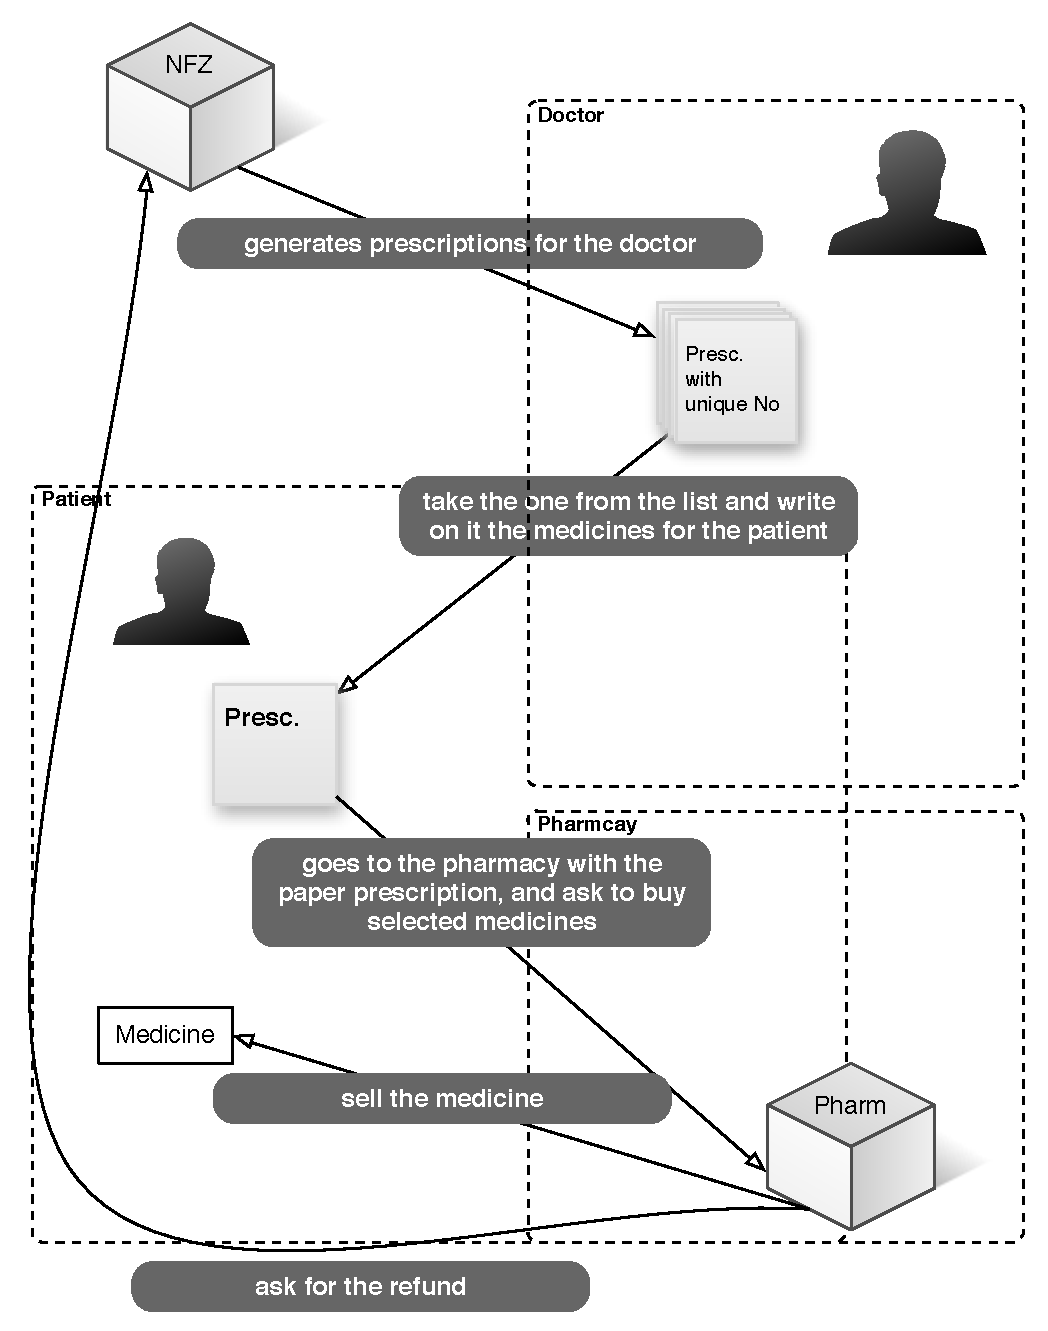
\includegraphics[scale=0.6]{cs.pdf}
    \caption{The main points of currently used system}
    \label{fig:mp_cs}
\end{figure} 

\chapter{\noun{Threats and Inconveniences}   }

The way prescriptions are currently processed is vulnerable to many threats, and brings many inconveniences. The most important ones are listed below.

\section{\noun{NFZ}}

\subsection{\noun{Defraudation}}

Significant amount of money is being defrauded from NFZ because the
current system does not verify if the patient himself has bought the
medicine or the pharmacists has made a false call for the medicine
having some patient's prescription, prepared by the doctor (who is
also a part of the defraudation scheme).

\section{\noun{Patient}}

\subsection{\noun{Losing a prescription}}
The patient can lose the prescription and he cannot buy the medicines,
even if they are life-saving, he has to go to the doctor again and
ask for the new prescription.

If someone finds lost prescription, he can buy this medicines; what is more, this person
can get to know, who takes which medicines and in this way, he can
get to know, what is wrong with the person described on the prescription.

\section{\noun{Pharmacy}}

\subsection{\noun{Refundation delay}}
The pharmacy has to wait long time to refund costs for the medicines
from NFZ.

\subsection{\noun{Prescriptions with mistakes}}
Prescription tend to contain mistakes which makes it useless. In this situation the patient has to go to the doctor again so it's fixed.

\section{\noun{System}}

\subsection{\noun{Prescription forgery}}
Patient can try to copy the prescription and try to buy the medicines
few times in different pharmacies.

\subsection{\noun{ Pretending that prescription was lost}}
Patient can claim that he has lost his prescription and ask the
doctor to give him another one. Then he can buy the medicines twice.

\chapter{\noun{The main objectives}   }

The main objectives of our new design of the pharmacy module is to limit the impact of the threats listed above and improve the user-friendliness. 

	\textbf{ The patient} has to be sure that his sensitive data is stored in a secure way, and unauthorized person cannot get to know anything about his medicines and illnesses. \textbf{The pharmacist} has to be sure that he sells the right medicines only for the right patient. \textbf{The refund process} should be quicker and easier. \textbf{The} possibility of making \textbf{mistakes} on the prescription should be eliminated. \textbf{The} number of \textbf{defraudations} should be significantly limited.






\chapter{\noun{Environment Description and Data Flows}   }


All the pharmacies which will be using our system must have broadband internet access, two smart card readers and two terminals: one for a pharmacist and one for a customer. The terminals apart from displaying the data need to handle all the confirmation actions on both sides. \newline
Pharmacists and pharmacies’ customers need to have valid smart cards which store their identification data (names, surnames, PESEL numbers and digital certificates). All the certificates must be given by a defined certification authority and renewed when necessary.


\textbf{\noun{Scenario}}

\begin{enumerate}
  \item Customer inserts his card into the reader and enters PIN number.
  \begin{enumerate}
	\item System checks whether PIN is correct (if it is not, an appropriate message is displayed and the process cannot be continued).
  \end{enumerate}
  \item Terminal displays list of active prescriptions to both buyer and pharmacist.
  \item Buyer selects prescriptions to buy.
  \item Pharmacist inserts his card into his reader and authenticates himself to the system (assuming that the card is not already inserted).
  \begin{enumerate}
	\item  If authentication is not possible (eg. card of the pharmacist is invalid), an appropriate error message appears on the screen and the process can't be continued.
  \end{enumerate}
  \item The pharmacist marks prescriptions selected by the customers as 'to be bought'.
  \item System checks whether prescriptions have already been bought (in case someone tampers with the card).
  \item System verifies validity of prescriptions (expiration date, credentials of the doctor etc.)
 \begin{enumerate}
	\item If some prescriptions are invalid, an appropriate message appears on the screen and system marks the prescriptions as 'invalid'.
  \end{enumerate}
  \item  If the drug from the prescription is not available (or the buyer does not want it for some reason), pharmacist can instead sell a substitute. For that, he is able to write information about selling a substitute to the system.
  \item Buyer confirms the prescriptions to be bought (including possible substitute replacements).
  \item Pharmacist gives the drugs to the buyer, confirms the selling and the system marks the prescriptions as 'bought'.
  \item  Buyer takes the drugs and removes his card from the reader.
\end{enumerate}

 If before step 10 either card is removed from the reader, process is aborted and initial state of the prescriptions does not change.

\begin{figure}
    \centering
    \hspace*{-1.2in}
    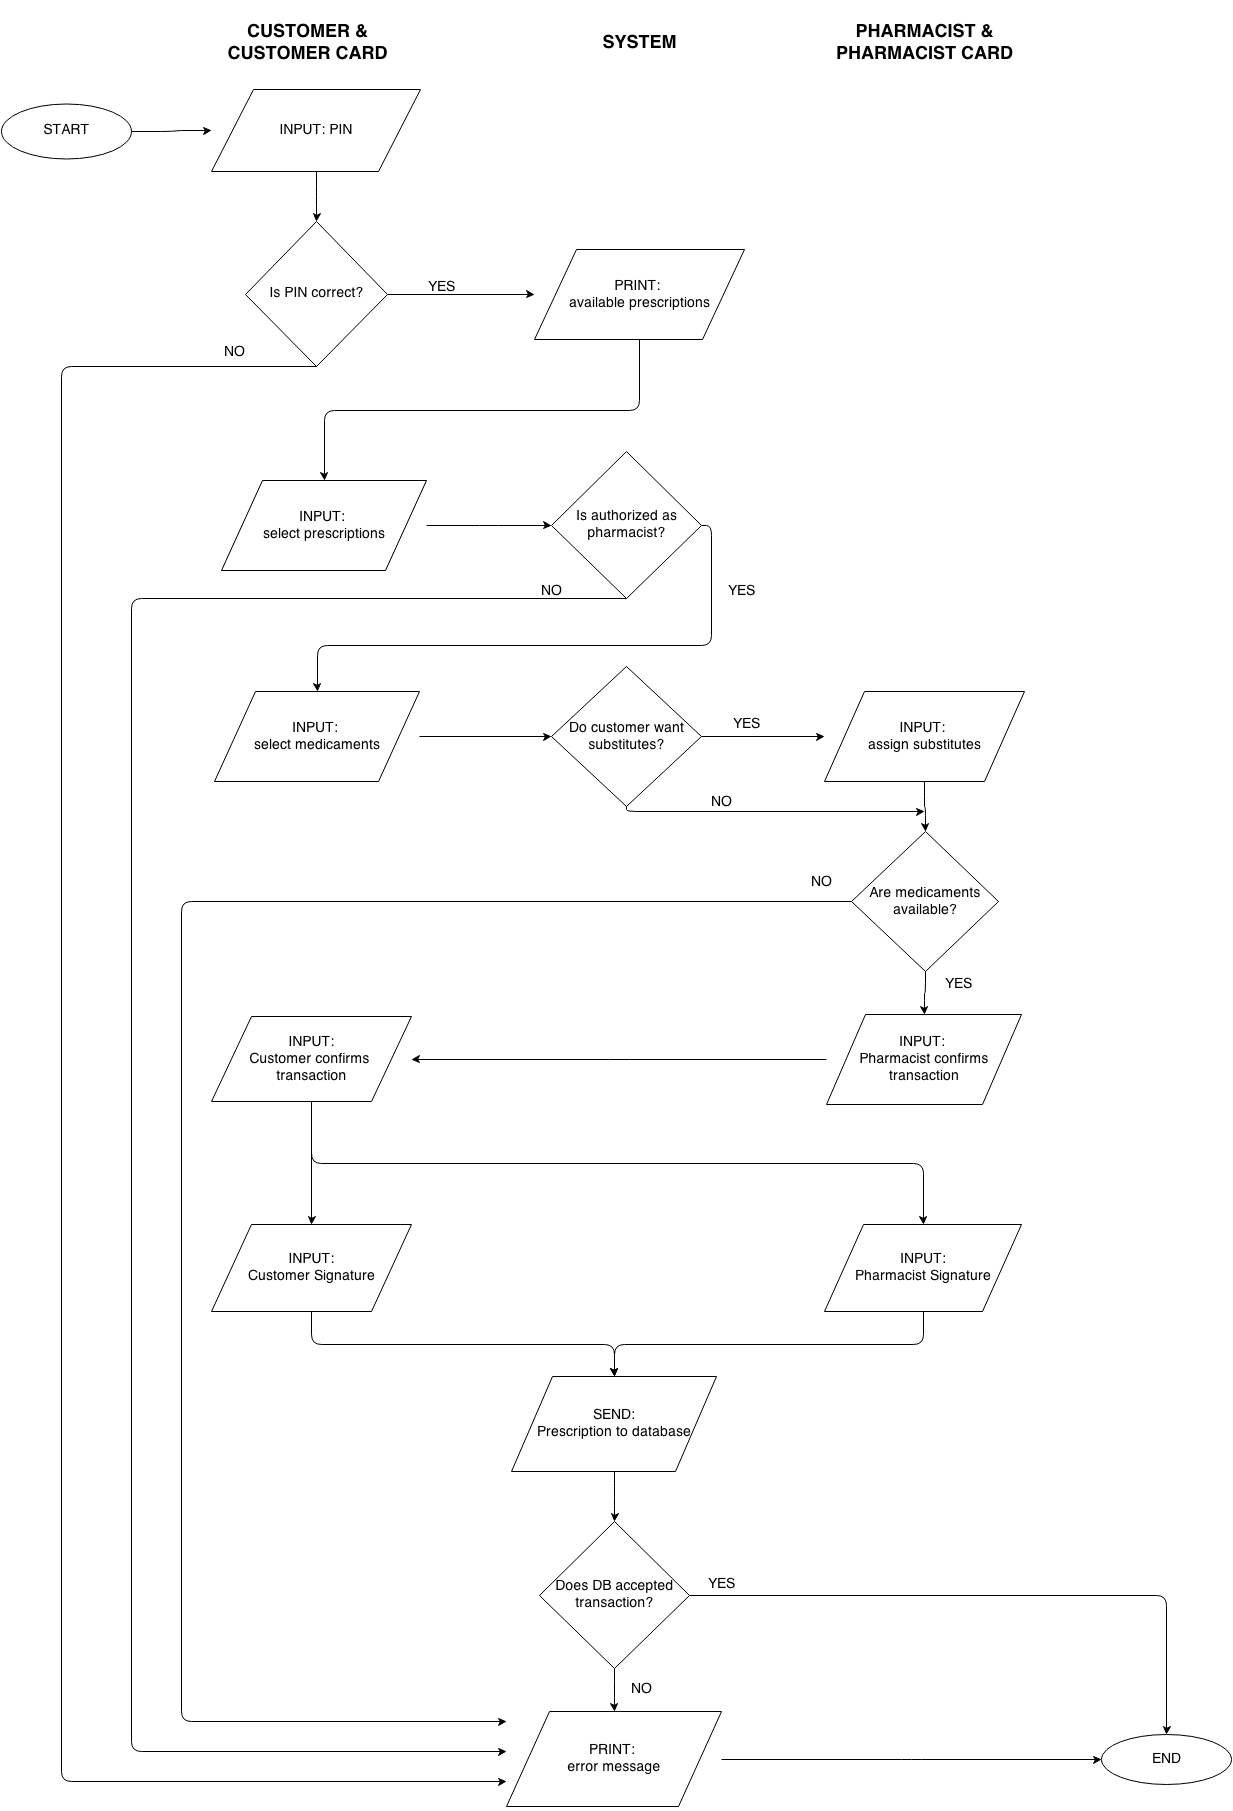
\includegraphics[width=0.98\textheight]{flow-chart.png}
    \caption{Flow chart}
    \label{fig:flowchart}
\end{figure} 


\chapter{\noun{Use cases}   }
In his chapter we present sequence diagram of the actions performed in the range of Pharmacy Module. Each step is detailed described. Not all actions are strongly required - sometimes it should depend on the security level requirement and budget possibilities. 

The first step is communication initialization. Actions performed in this step by the system elements are presented on the figure \ref{fig:s_q_step_1}
\begin{figure}	
	\hspace*{-1.5in}
    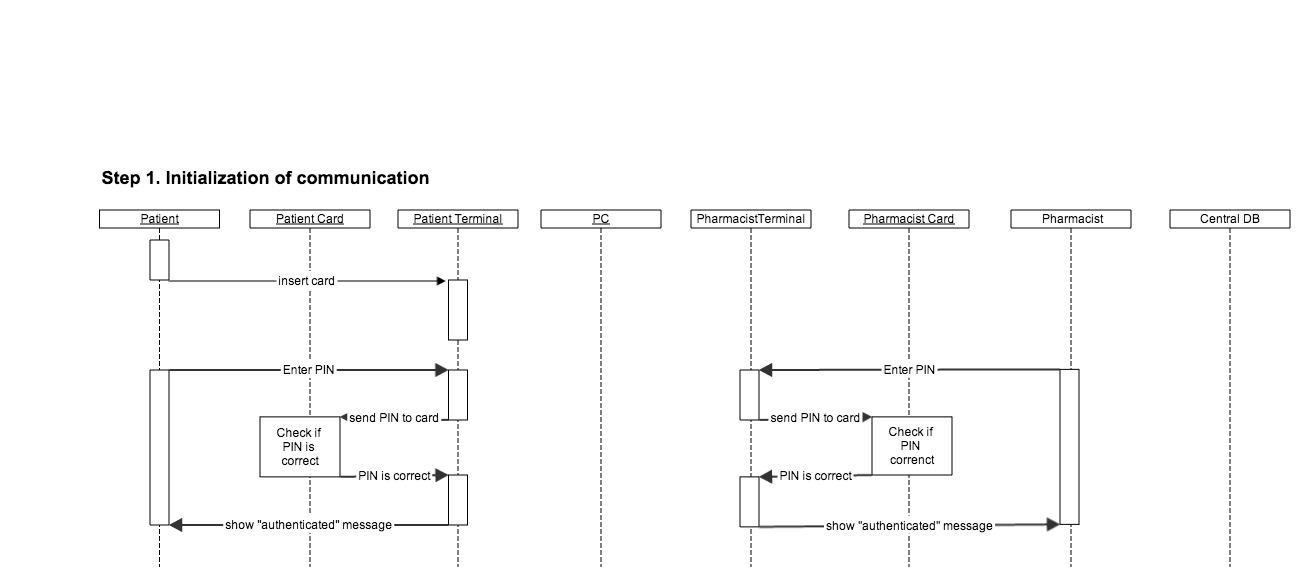
\includegraphics[scale=0.45]{s_d_1.png}
    \caption{Sequence diagram - step 1}
    \label{fig:s_q_step_1}
\end{figure} 

At the beginning, the patient put his personal card to the terminal and he enter the PIN as usual e.g. in the ATM. If the PIN is correct, the user can show appropriate message on the terminal screen. Also the pharmacist have to use his card and enter the PIN in the second terminal. Then, the system is ready to work. 

Necessity to use the PIN by the user and the pharmacist prevents the risk the situation, when e.g. the card was stolen or lost.


\begin{figure}	
	\hspace*{-1.5in}
    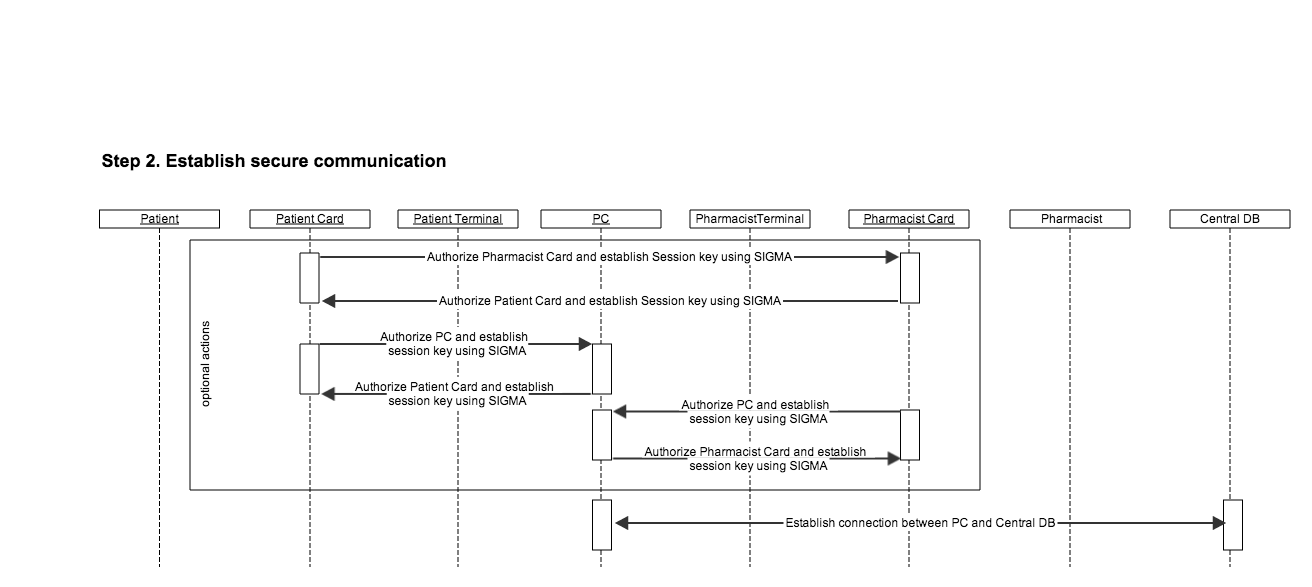
\includegraphics[scale=0.45]{s_d_2.png}
    \caption{Sequence diagram - step 2}
    \label{fig:s_q_step_2}
\end{figure} 

The second step, presented on the figure \ref{fig:s_q_step_2}, contains actions related with establishing secure communication ways between the system parties. There are marked the actions, which are optional and are not required for the system to work properly. Establishing secure communication between the cards allows the participant to be sure, that the patient ant pharmacist cards are not the fake cards and they are authenticated to each other.
Similarly, suing the SIGMA protocol between the card (patient or pharmacist) and the application installed on the PC, allows to authorization the application by the card and the card by the application. However. this two sub-steps can be implement, if the very-high level of the security from this point of view is required. 

\begin{figure}	
	\hspace*{-1.5in}
    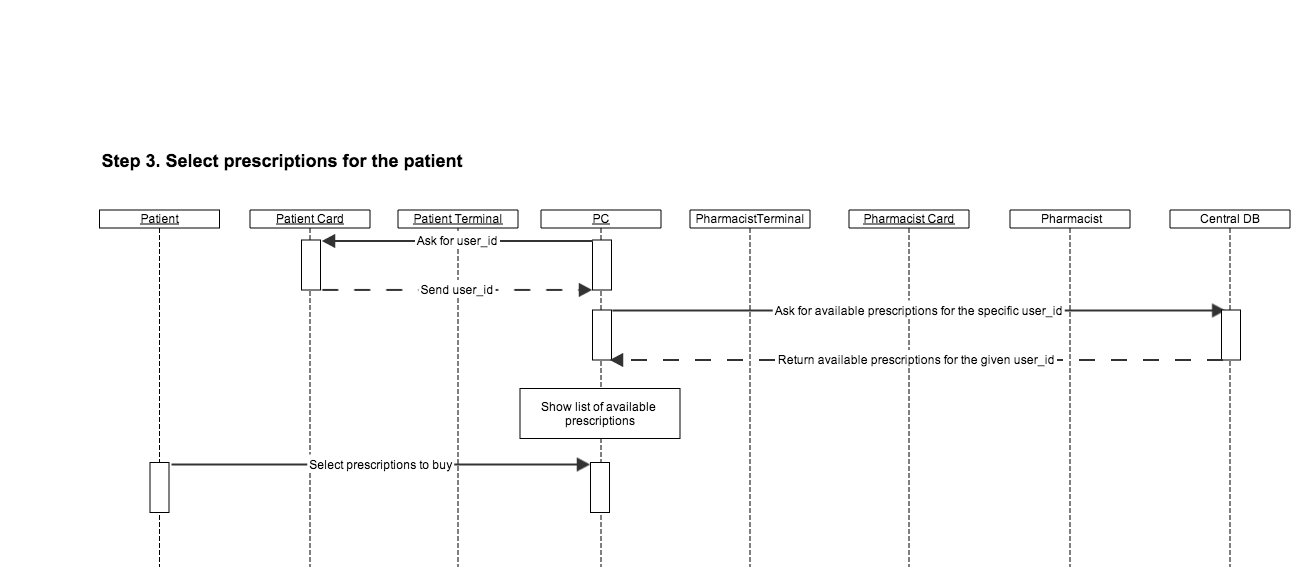
\includegraphics[scale=0.45]{s_d_3.png}
    \caption{Sequence diagram - step 3}
    \label{fig:s_q_step_3}
\end{figure} 

The figure \ref{fig:s_q_step_3} presents the point in the protocol, when the prescriptions for the user are download from the Central Database and are shown on the screen. Then, the patient have the possibility to select one or more of them to realize them. The data of the user are saved inside the patient card, so the application have to get this data to download appropriate prescriptions. 

\begin{figure}	
	\hspace*{-1.5in}
    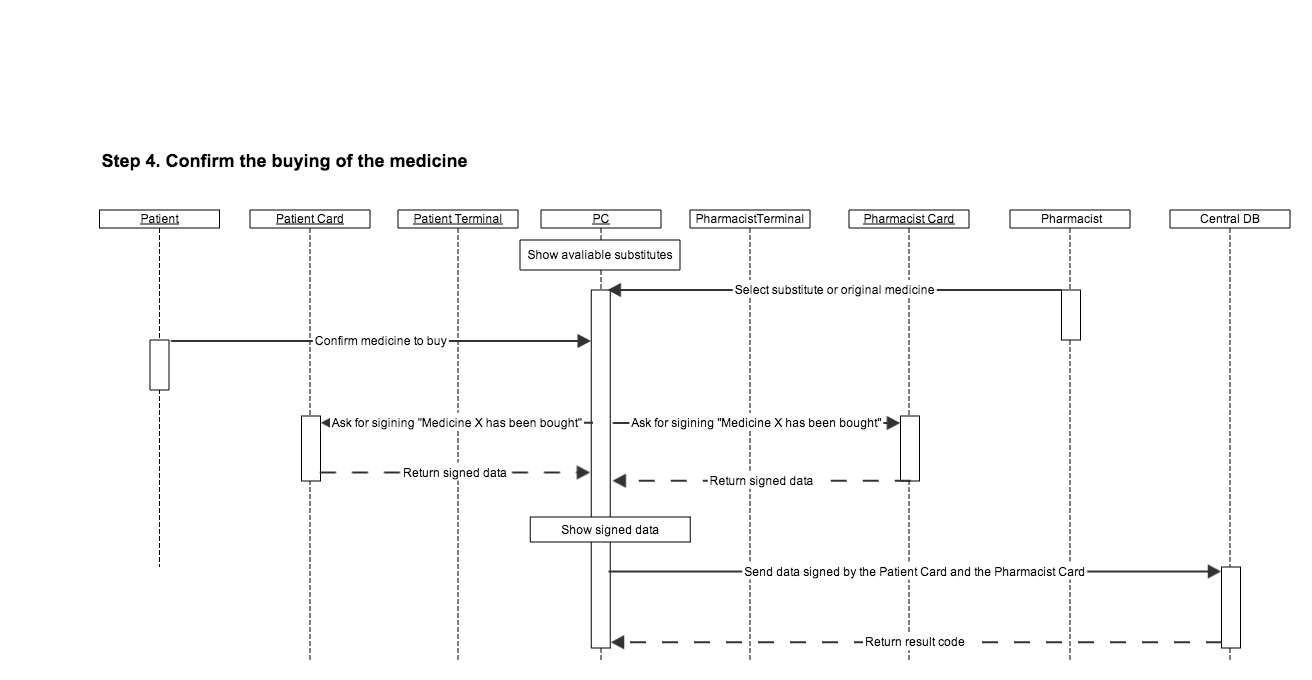
\includegraphics[scale=0.45]{s_d_4.png}
    \caption{Sequence diagram - step 4}
    \label{fig:s_q_step_4}
\end{figure} 






%-----------------------------------------------------------
%\addcontentsline{toc}{chapter}{\numberline{}Bibliography}
%\include{biblio}
%-----------------------------------------------------------

%-----------------------------------------------------------
\end{document}
